\chapter{Технологическая часть}

В данной части представляются выбор средств реализации и исходный код программы, описываются организация классов в программе и её интерфейс.

\section{Средства реализации программы}

В качестве языка программирования для реализации данной курсовой работы был выбран $C\#$ по следующим причинам~\cite{lit9}:
\begin{itemize}[label=--]
	\item в стандартной библиотеке $C\#$ присутствуют необходимые структуры и классы, выбранные по результатам проектирования;
	\item поддержка объектно-ориентированного программирования;
	\item поддержка механизма многопоточности.
\end{itemize}

Для измерения процессорного времени выполнения кода был выбран класс \textit{Stopwatch}, который находится в пространстве имен \textit{System.Diagnostics}~\cite{lit10}.

\section{Структура программы}

Разработанная программа состоит из следующих классов:
\begin{enumerate}
	\item управляющий класс:
	\begin{itemize}[label=--]
		\item \textit{Program} -- точка входа в программу.
	\end{itemize}
	\begin{figure}[h] 
		\centering
		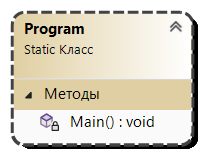
\includegraphics[width=0.2\textwidth]{images/main-class.png}
		\caption{Управляющий класс} 
		\label{fig:main-class} 
	\end{figure}
	\item классы интерфейса:
	\begin{itemize}[label=--]
		\item \textit{Form1} -- главное окно программы;
		\item \textit{DialogEdit} -- окно редактирования модели;
		\item \textit{ErrorMessage} -- окно, содержащее сообщение об ошибке.
	\end{itemize}
	\clearpage
	\begin{figure}[h] 
		\centering
		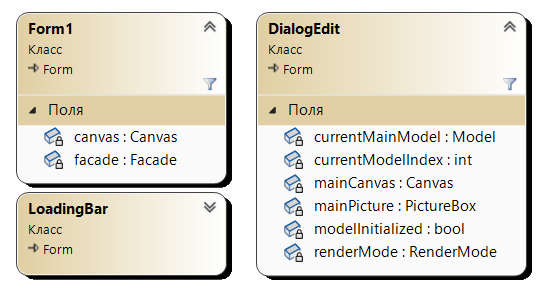
\includegraphics[width=0.5\textwidth]{images/interface-class.png}
		\caption{Классы интерфейса} 
		\label{fig:interface-class} 
	\end{figure}
	\item классы инкапсуляции действий:
	\begin{itemize}[label=--]
		\item \textit{Command} -- базовый класс команды для выполнения;
		\item \textit{SceneCommand} -- базовый класс команды для обработки сцены;
		\item \textit{CameraCommand} -- базовый класс команды для обработки камеры;
		\item \textit{DrawsCommand} -- базовый класс команды для обработки экрана;
		\item \textit{TransformationCommand} -- базовый класс команды для преобразований объектов;
		\item \textit{FormCommand} -- базовый класс команды для обработки интерфейса.
	\end{itemize}
	\begin{figure}[h] 
		\centering
		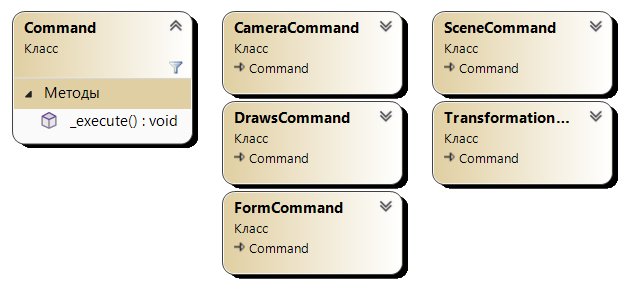
\includegraphics[width=0.6\textwidth]{images/commands-class.png}
		\caption{Классы инкапсуляции действий} 
		\label{fig:commands-class} 
	\end{figure}
	\item классы обработки команд:
	\begin{itemize}[label=--]
		\item \textit{Facade} -- единый интерфейс для обработки команд;
		\item \textit{SceneManager} -- обработчик команд, работающих со сценой;
		\item \textit{DrawManager} -- обработчик команд, работающих с экраном;
		\item \textit{TransformationManager} -- обработчик команд, преобразовывающих объекты;
		\item \textit{FormManager} -- обработчик команд, работающих с интерфейсом.
	\end{itemize}
	\begin{figure}[h] 
		\centering
		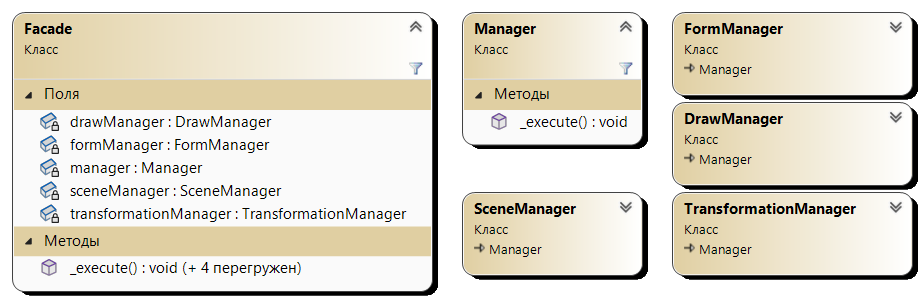
\includegraphics[width=0.8\textwidth]{images/commandsprocessors-class.png}
		\caption{Классы обработки команд} 
		\label{fig:commandsprocessors-class} 
	\end{figure}
	\item классы взаимодействия со сценой:
	\begin{itemize}[label=--]
		\item \textit{Canvas} -- менеджер изображения на экране;
		\item \textit{Scene} -- менеджер трехмерной сцены;
		\item \textit{ViewingSystem} -- менеджер просмотра сцены.
	\end{itemize}
	\begin{figure}[h] 
		\centering
		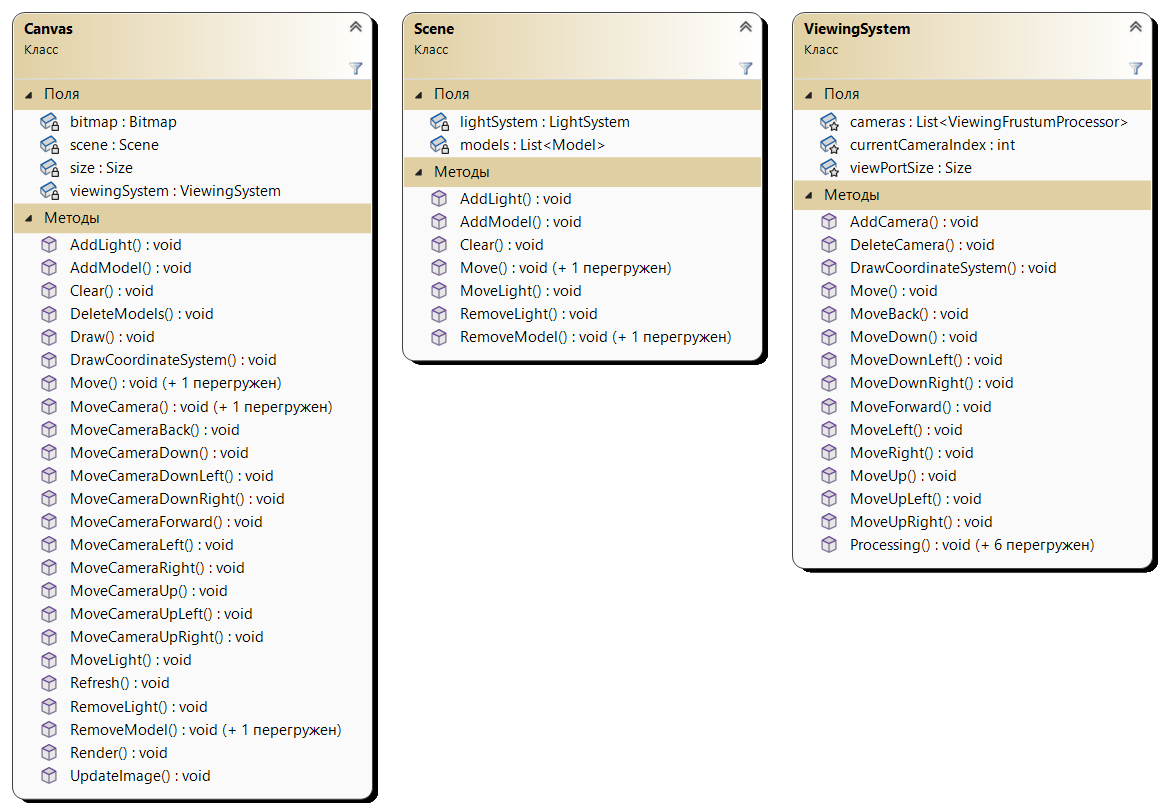
\includegraphics[width=0.8\textwidth]{images/canvas-class.png}
		\caption{Классы взаимодействия со сценой} 
		\label{fig:canvas-class} 
	\end{figure}
	\item классы представления света:
	\begin{itemize}[label=--]
		\item \textit{LightSystem} -- менеджер источников света;
		\item \textit{Light} -- источник света.
	\end{itemize}
	\clearpage
	\begin{figure}[h] 
		\centering
		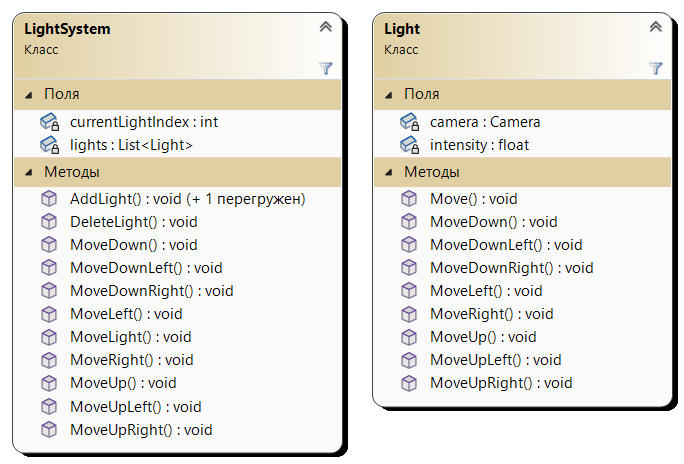
\includegraphics[width=0.6\textwidth]{images/light-class.png}
		\caption{Классы представления света} 
		\label{fig:light-class} 
	\end{figure}
	\item классы представления моделей:
	\begin{itemize}[label=--]
		\item \textit{Model} -- базовый класс многогранной модели;
		\item \textit{Cube} -- куб;
		\item \textit{DirectPrism} -- прямая призма;
		\item \textit{Pyramid} -- треугольная пирамида.
	\end{itemize}
	\begin{figure}[h] 
		\centering
		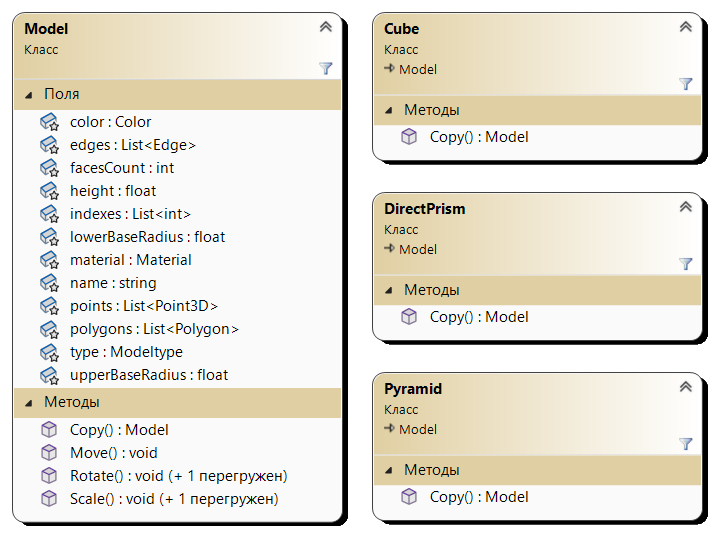
\includegraphics[width=0.6\textwidth]{images/model-class.png}
		\caption{Классы представления моделей} 
		\label{fig:model-class} 
	\end{figure}
	\item классы представления камеры:
	\begin{itemize}[label=--]
		\item \textit{Camera} -- камера;
		\item \textit{ViewingFrustum} -- камера, учитывающая видимое пространство и визуализирующая сцену с использованием перспективных преобразований;
		\item \textit{ViewingFrustumZBuffer} -- камера, учитывающая видимое пространство, визуализирующая сцену с использованием перспективных преобразований и удалением невидимых линий и поверхностей;
		\item \textit{ViewingFrustumParallelZBuffer} -- камера \textit{ViewingFrustumZBuffer}, реализованная с использованием параллельных потоков;
		\item \textit{ViewingFrustumPhongShading} -- камера, учитывающая видимое пространство, визуализирующая сцену с использованием перспективных преобразований, удалением невидимых линий и поверхностей и расчетом освещенности объектов;
		\item \textit{ViewingFrustumParallelPhongShading} -- камера \newline \textit{ViewingFrustumPhongShading}, реализованная с использованием параллельных потоков;
		\item \textit{ViewingFrustumShadows} -- камера, учитывающая видимое пространство, визуализирующая сцену с использованием перспективных преобразований, удалением невидимых линий и поверхностей, расчетом освещенности объектов и возникающих теней;
		\item \textit{ViewingFrustumParallelShadows} -- камера \textit{ViewingFrustumShadows}, реализованная с использованием параллельных потоков;
		\item \textit{ViewingFrustumProcessor} -- камера с многорежимной визуализацией сцены.
	\end{itemize}
	\clearpage
	\begin{figure}[h] 
		\centering
		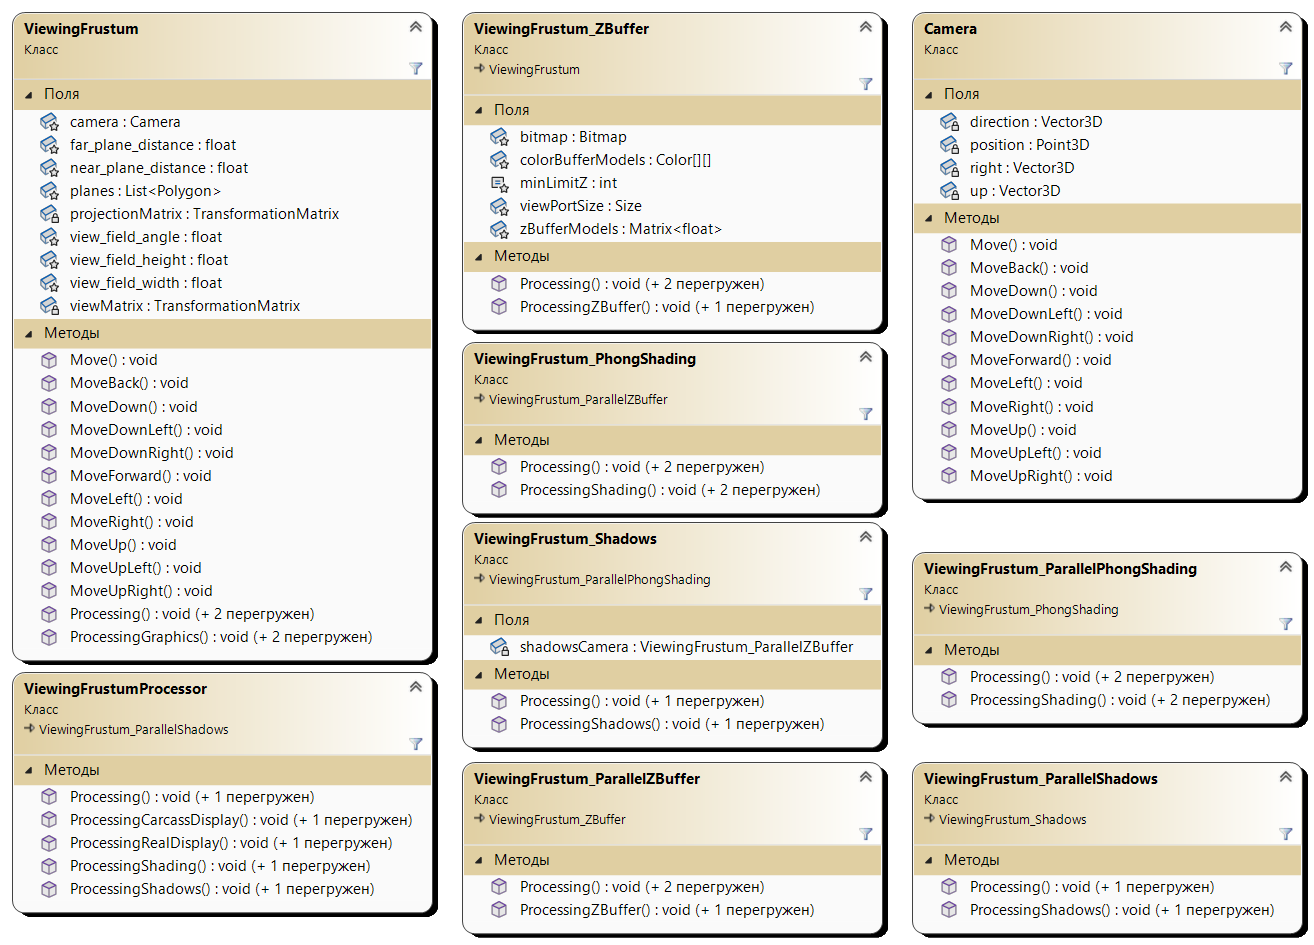
\includegraphics[width=1\textwidth]{images/camera-class.png}
		\caption{Классы представления камеры} 
		\label{fig:camera-class} 
	\end{figure}
	\item классы афинных преобразований:
	\begin{itemize}[label=--]
		\item \textit{Transformation} -- базовый класс афинного преобразования;
		\item \textit{Move} -- перемещение;
		\item \textit{Rotate} -- поворот;
		\item \textit{Scale} -- масштабирование.
	\end{itemize}
	\begin{figure}[h] 
		\centering
		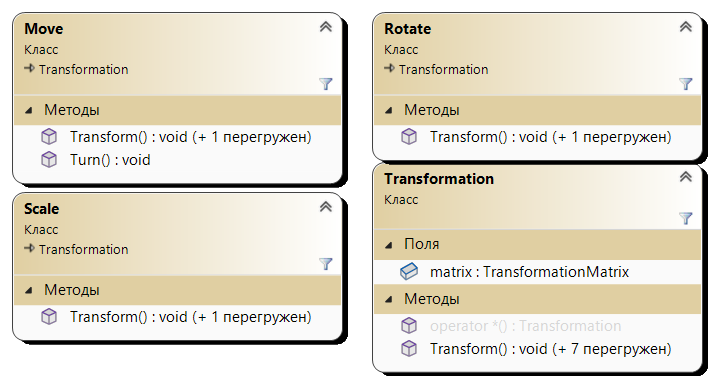
\includegraphics[width=0.532\textwidth]{images/transformation-class.png}
		\caption{Классы аффинных преобразований} 
		\label{fig:transformation-class} 
	\end{figure}
	\item математические классы:
	\begin{itemize}[label=--]
		\item \textit{Matrix} -- матрица;
		\item \textit{TransformationMatrix} -- матрица афинного преобразования;
		\item \textit{Vector3D} -- трехмерный вектор.
	\end{itemize}
	\begin{figure}[h] 
		\centering
		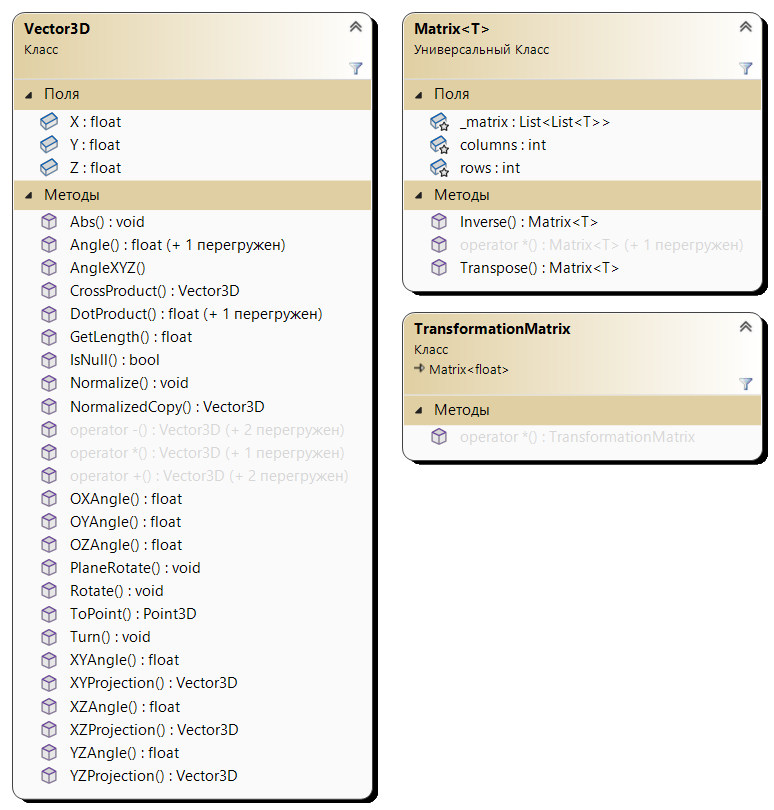
\includegraphics[width=0.7\textwidth]{images/math-class.png}
		\caption{Математические классы} 
		\label{fig:math-class} 
	\end{figure}
\end{enumerate}

Исходный код реализованной программы доступен в открытом сетевом репозитории~\cite{lit11}.

\section{Интерфейс программы}

При запуске программы пользователю демонстрируется пустая сцена и панель, содержащая вкладки <<Главная>> и <<Вид>>. Вкладка <<Главная>> позволяет пользователю добавлять примитивы на сцену, редактировать добавленные примитивы, очищать сцену и изменять режим отображения сцены. Вкладка <<Вид>> позволяет пользователю перемещать камеру, изменять спектральные характеристики и положение источника света.

\begin{figure}[h] 
	\centering
	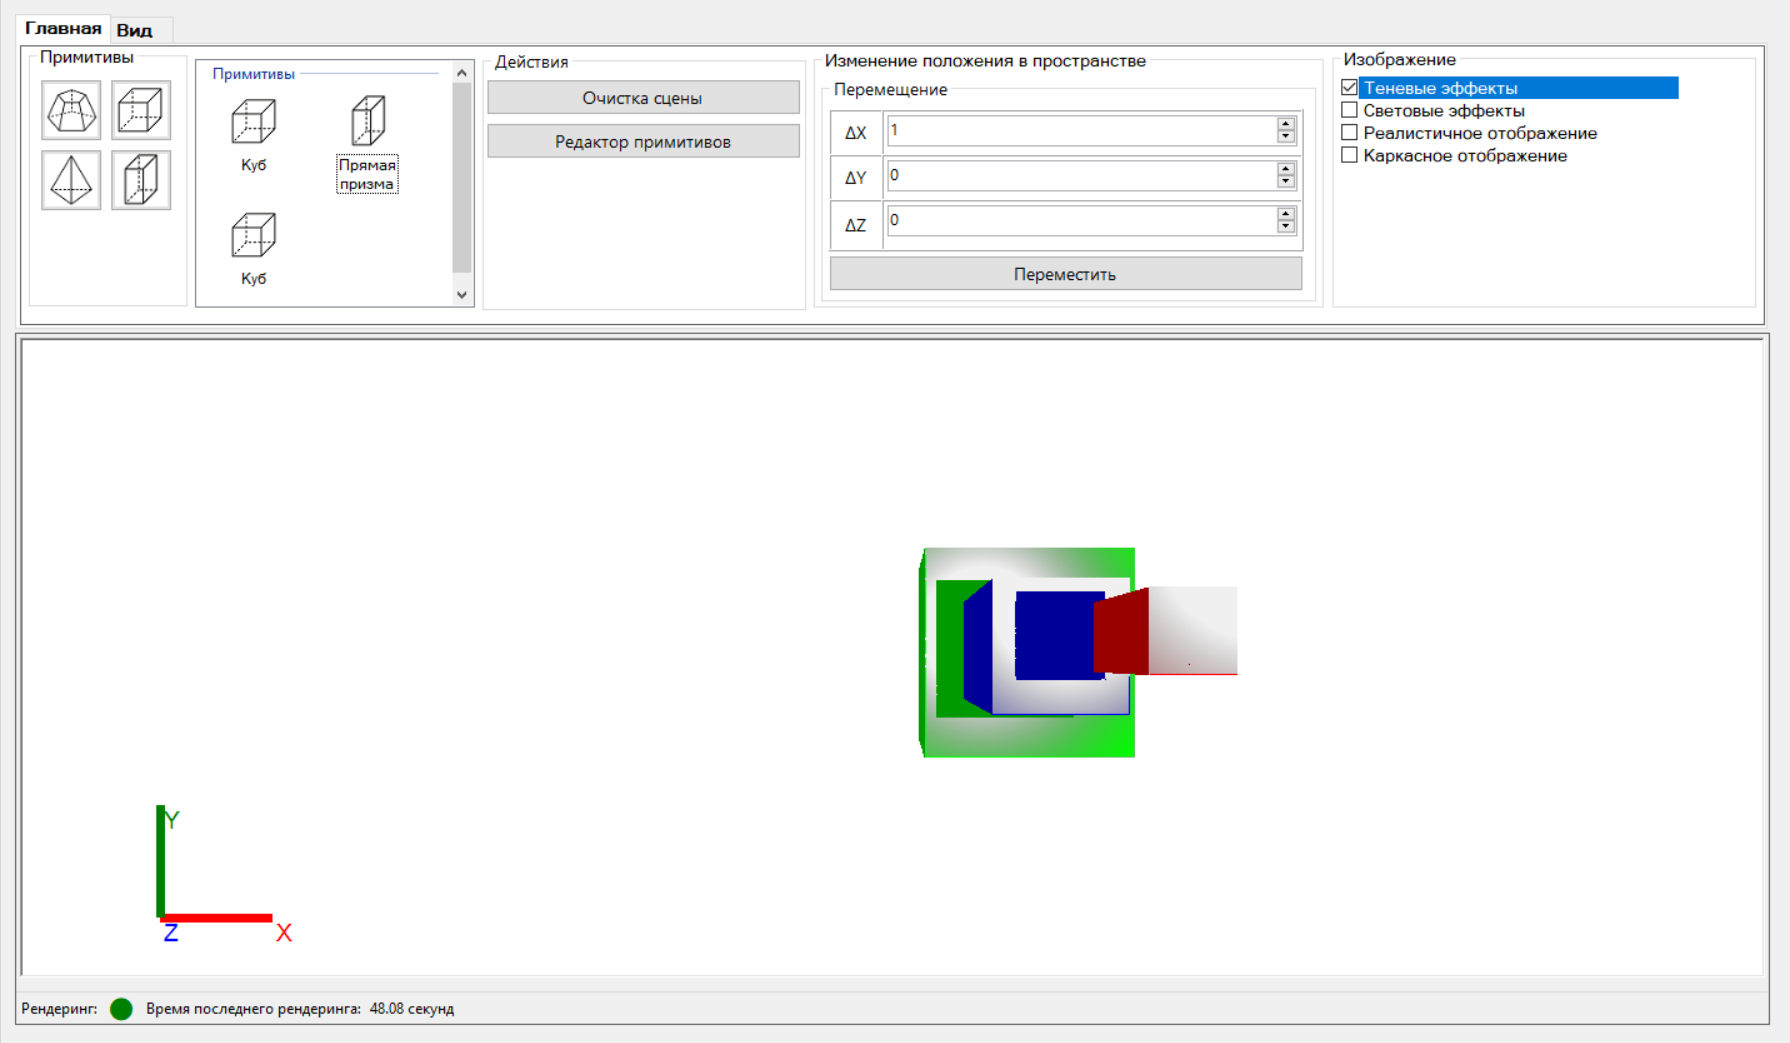
\includegraphics[width=1\textwidth]{images/main-interface.png}
	\caption{Интерфейс главного окна программы во вкладке <<Главная>>} 
	\label{fig:main-interface} 
\end{figure}

\begin{figure}[h] 
	\centering
	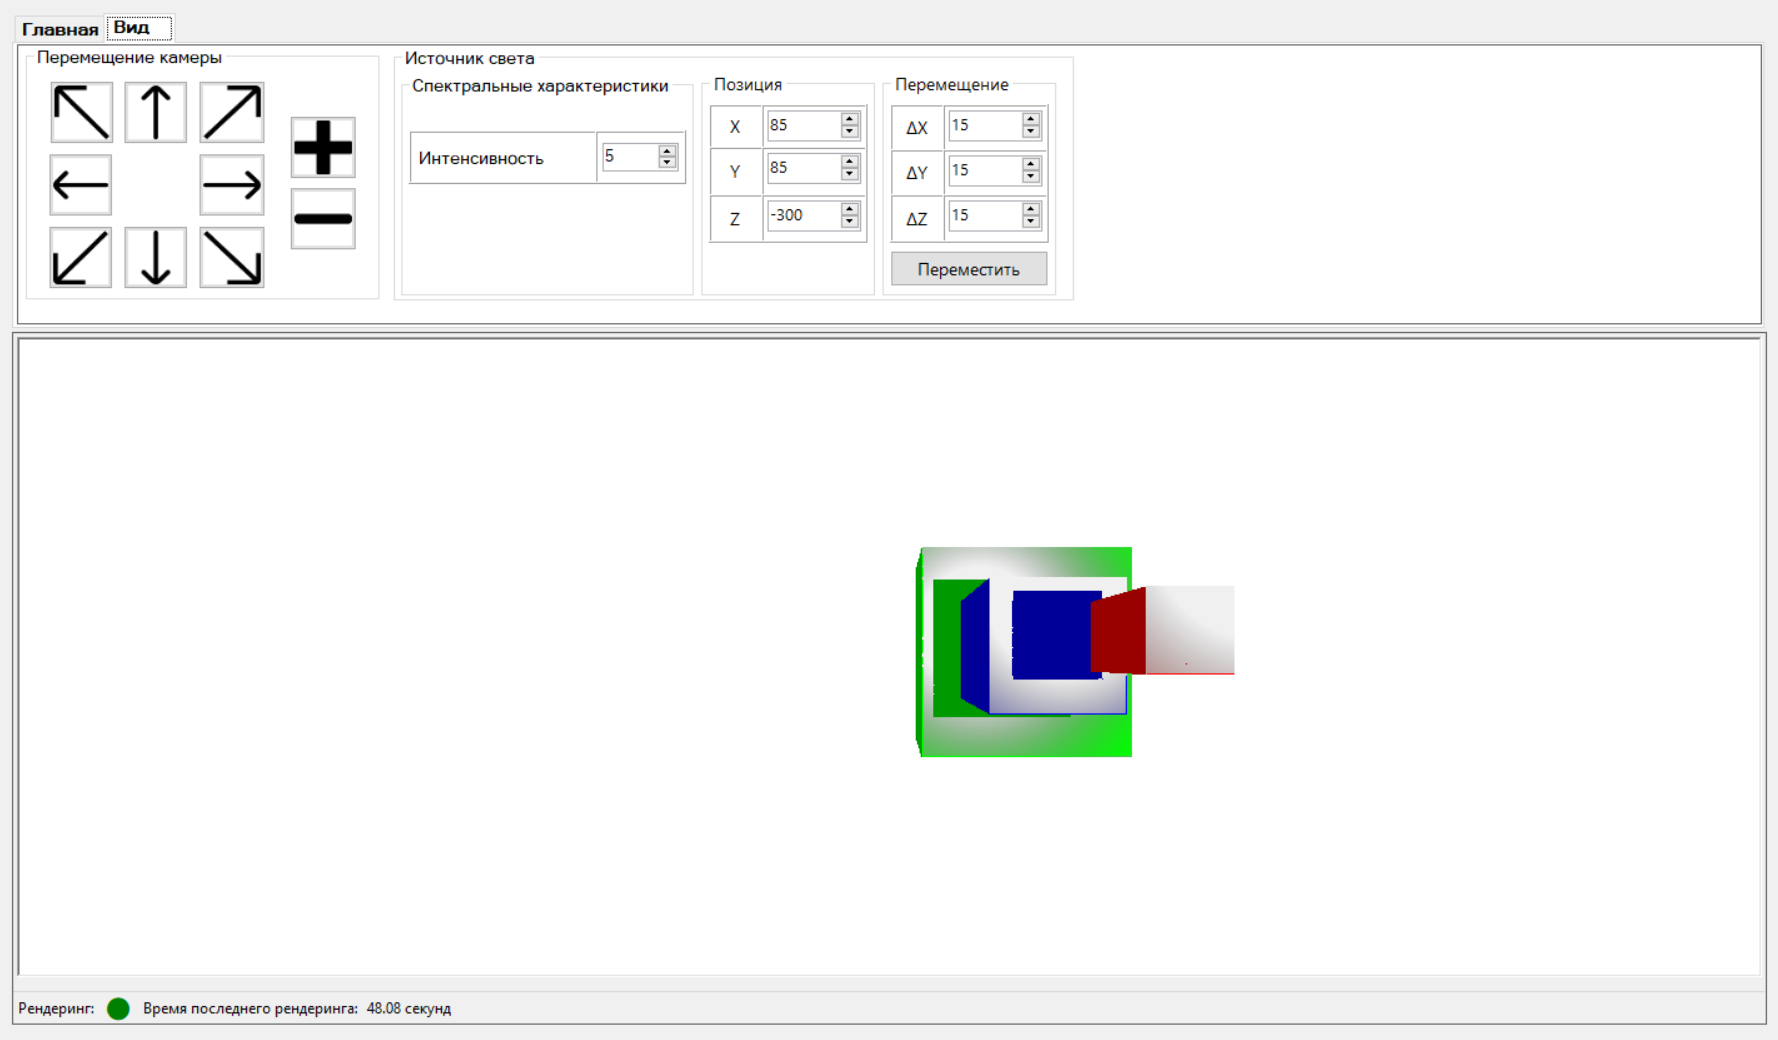
\includegraphics[width=1\textwidth]{images/view-interface.png}
	\caption{Интерфейс главного окна программы во вкладке <<Вид>>} 
	\label{fig:view-interface} 
\end{figure}

\clearpage

\begin{enumerate}
	\item вкладка <<Главная>> содержит:
	\begin{itemize}[label=--]
		\item группу <<Примитивы>>, содержащую 4 кнопки, отвечающие за добавление на сцену многогранника, куба, прямой призмы и треугольной пирамиды соответственно;
		\begin{figure}[h] 
			\centering
			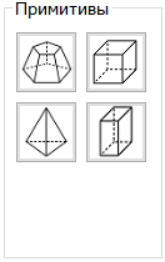
\includegraphics[width=0.15\textwidth]{images/primitives-buttons.png}
			\caption{Группа <<Примитивы>>} 
			\label{fig:primitives-buttons} 
		\end{figure}
		\item коллекцию <<Примитивы>>, отображающую присутствующие примитивы на сцене и позволяющую выбирать изменяемый примитив;
		\begin{figure}[h] 
			\centering
			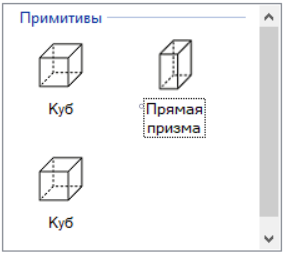
\includegraphics[width=0.25\textwidth]{images/primitives-list.png}
			\caption{Коллекция <<Примитивы>>} 
			\label{fig:primitives-list} 
		\end{figure}
		\item группу <<Действия>>, содержащую две кнопки: <<Очистить>>, очищающую сцену от добавленных примитивов, <<Редактор примитивов>>, открывающую окно редактирования примитивов на сцене;
		\begin{figure}[h] 
			\centering
			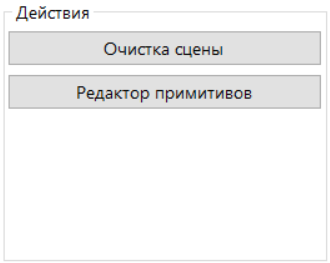
\includegraphics[width=0.3\textwidth]{images/actions.png}
			\caption{Группа <<Действия>>} 
			\label{fig:actions} 
		\end{figure}
		\item группу <<Изменение положения в пространстве>>, содержащую группу <<Перемещение>>, позволяющую задавать параметры перемещения примитива и перемещать его нажатием кнопки <<Переместить>>;
		\begin{figure}[h] 
			\centering
			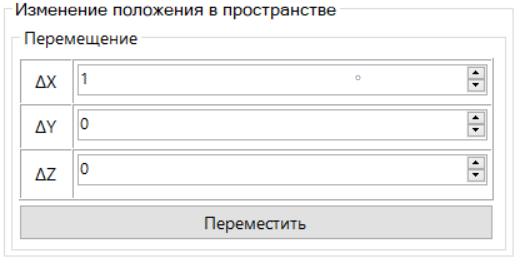
\includegraphics[width=0.45\textwidth]{images/move.png}
			\caption{Группа <<Изменение положения в пространстве>>} 
			\label{fig:move} 
		\end{figure}
		\item группу <<Изображение>>, содержащую список с возможностью выбора текущего режима отображения сцены между <<Теневыми эффектами>>, <<Световыми эффектами>>, <<Реалистичным отображением>> и <<Каркасным отображением>>.
		\begin{figure}[h] 
			\centering
			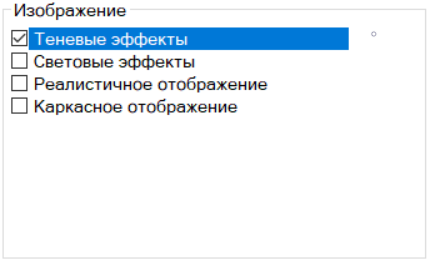
\includegraphics[width=0.45\textwidth]{images/mods.png}
			\caption{Группа <<Изображение>>} 
			\label{fig:mods} 
		\end{figure}
	\end{itemize}
	\item вкладка <<Вид>> содержит:
	\begin{itemize}[label=--]
		\item группу <<Перемещение камеры>>, содержащую 10 кнопок и позволяющую переместить камеру нажатием на соответствующую кнопку;
		\clearpage
		\begin{figure}[h] 
			\centering
			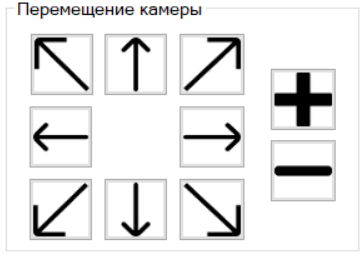
\includegraphics[width=0.35\textwidth]{images/camera-move.png}
			\caption{Группа <<Перемещение камеры>>} 
			\label{fig:camera-move} 
		\end{figure}
		\item группу <<Источник света>>, которая содержит группы <<Спектральные характеристики>>, <<Позиция>> и <<Перемещение>>, позволяющие задавать интенсивность потока света, испускаемого источником, изменять его позицию на сцене, определять параметры перемещения и перемещать нажатием кнопки <<Переместить>> соответственно.
		\begin{figure}[h] 
			\centering
			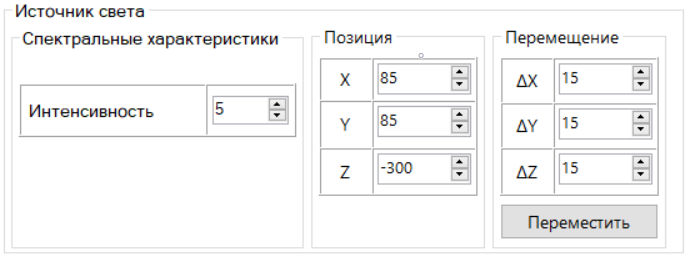
\includegraphics[width=0.65\textwidth]{images/light.png}
			\caption{Группа <<Источник света>>} 
			\label{fig:light} 
		\end{figure}
	\end{itemize}
\end{enumerate}

При нажатии на кнопку <<Редактор примитивов>>, расположенной в группе <<Действия>> вкладки <<Главная>> (рис.~\ref{fig:actions}) будет открыто окно редактирования примитивов, в котором можно изменять их геометрические, спектральные, цветовые и информационные параметры. Для каждого из примитивов определен свой набор изменяемых геометрических параметров, потому некоторые параметы могут быть недоступны для изменения.
\clearpage
\begin{figure}[h] 
	\centering
	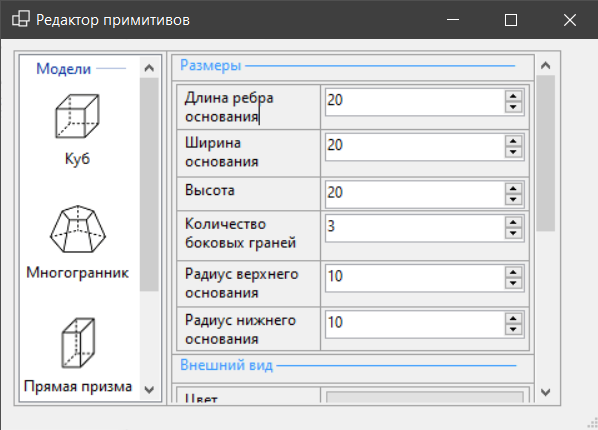
\includegraphics[width=0.65\textwidth]{images/model-editor1.png}
	\caption{Интерфейс окна редактирования примитивов (часть 1)} 
	\label{fig:model-editor1} 
\end{figure}
\begin{figure}[h] 
	\centering
	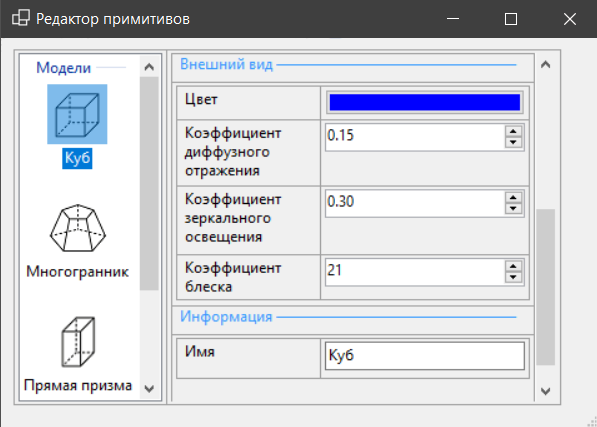
\includegraphics[width=0.65\textwidth]{images/model-editor2.png}
	\caption{Интерфейс окна редактирования примитивов (часть 2)} 
	\label{fig:model-editor2} 
\end{figure}

\section{Вывод}

В данной части быил представлены выбор средств реализации и исходный код программы, описаны организация классов в программе и её интерфейс.

\clearpage
